\onehalfspacing

\chapter{Choosing estimates for simulation parameters}

\label{chap:Chapter_4}

The algorithm described in the previous chapter; see Algorithm \ref{alg:algorithm}, for evolving dynamics of droplets from \Eqsref{eqn:DropletDiscretized} and dynamics of the background field dynamics from \Eqref{eqn:RD_dilute}, has several simulation parameters that need to be chosen wisely for an accurate and fast simulation.
In particular, from \figref{fig:schematics}, we see that we need to specify: a) Discretization $\dx$ of the background field volume fraction $\phiOut$, b) Shell thickness $\ell$ and c) Width $\ds$ of a shell sector.
Note that for $d=2,3$ dimensions, we respectively use $\ds \approx 2\pi R/N$ and $\ds \approx\sqrt{4 \pi R^2 / N}$; see \figref{fig:schematics}B.

While $\dx$ and $\ds$ are discretization parameters, where we expect better accuracy (and worse performance) for smaller values, the shell thickness $\ell$ is a simulation parameter that determines how the droplets interact with the background field and its effect is less obvious.
We first discuss the effects of each of the simulation parameter on the dynamics of droplets and the background field. 
We then choose suitable values for all three parameters ($\dx, \ell, \ds$) using a detailed simulation of the continuous model given by \Eqref{eqn:CHActive} as ground truth to be compared with simulations using the effective droplet model.

\begin{figure}[tb]
\centering
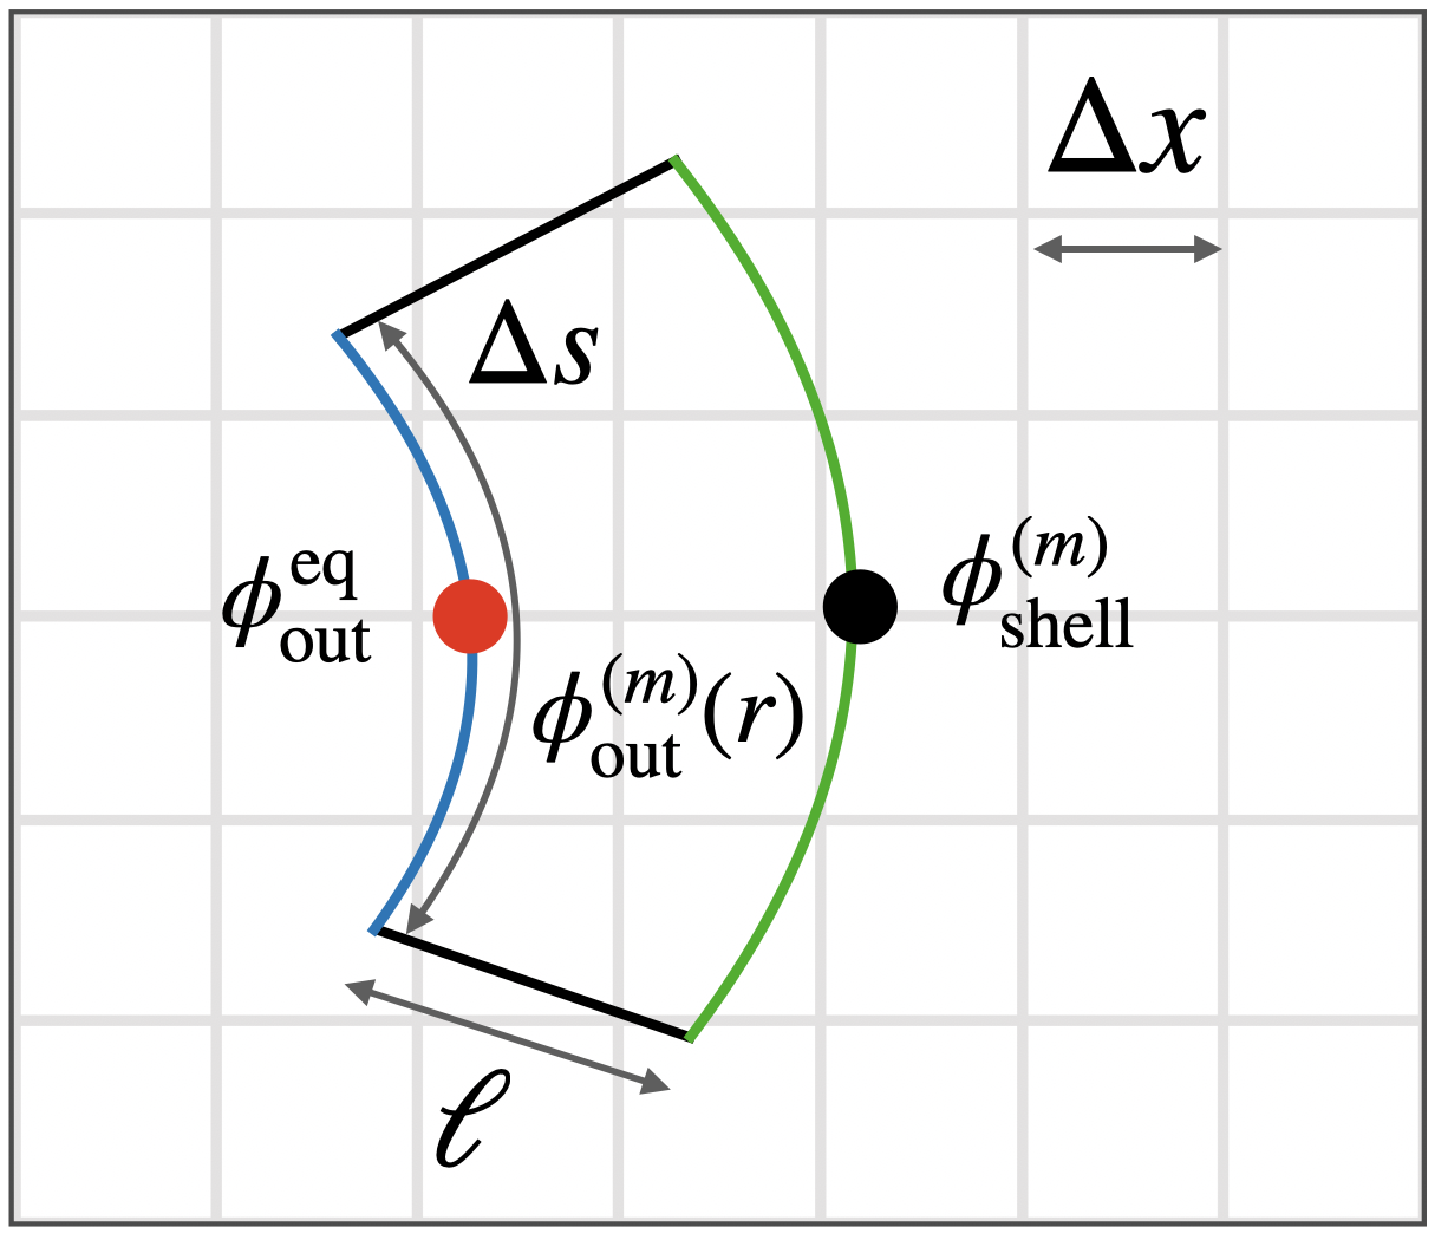
\includegraphics[scale=0.27]{MainContent/Figures/schematics_simulation_parameters.pdf}
\caption{
\textbf{Simulation parameters $\dx, \ell, \ds$ in the effective droplet model shown in a shell sector.}
$\dx$ is the resolution of the discretized background field $\phiOut$ and is an important parameter to capture it's dynamics described by \Eqref{eqn:RD_dilute}. 
$\ell$ and $\ds$
discretize the vicinity of the droplet into $N$ uniformly chosen sectors.
We solve for $\phiOut^{(m)}(r)$ inside the $m$-th shell sector from \Eqref{eqn:phi_out_in_shell} using the boundary conditions $\phiOut^{(m)}(R) = \phiEqOut$ and $\phiOut^{(m)}(R + \ell) = \phiShell^{(m)}$, which is estimated from a linear interpolation of the discretized background field $\phiOut$.
We then evaluate the fluxes $\jIn$; see \Eqref{eqn:flux_inside}, and $\jOut$; see Appendix \ref{sec:fluxes_inside_shell}, to calculate dynamics of droplets described by \Eqsref{eqn:DropletDiscretized}. 
}
\label{fig:schematics_simulation_parameters}
\end{figure}

\section{Grid discretization $\dx$}

The spatial discretization $\dx$; (see Fig. \ref{fig:schematics_simulation_parameters}), determines the resolution at which spatial variations of the background field $\phiOut$ are resolved.
Consequently, the choice of $\dx$ is based on the physics of the problem:

\begin{enumerate}
    \item If spatial variation in $\phiOut$ is negligible and a mean-field model is desired, $\dx$ can be arbitrarily large so that $\phiOut$ can vary only in time and little in space.
    
    \item If spatial variation of $\phiOut$ between droplets are important, $\dx$ needs to be smaller or equal than the mean droplet separation to resolve droplet-droplet interactions mediated through the background field $\phiOut$.
    
    \item External gradients that affect droplets; see Refs. \cite{Review2019,Weber2017,Lee2013,Bressloff2020,Bressloff_2020} can also play a role in determining the resolution of $\phiOut$, as $\dx$ needs to be on the order of the droplet radii, so spatial anisotropies can be resolved on the droplet level.
\end{enumerate}
To summarize, several competing length-scales of interest can exist such as the mean droplet radius, mean droplet-droplet separation distance, external gradients, reaction-diffusion length-scales; see Ref. \cite{Review2019} at which the resolution of $\phiOut$ is desired. 
Consequently, we fix $\Delta x$ based on the length-scale at which the resolution of $\phi_{\mathrm{out}}$ is needed.

\section{Annular shell thickness $\ell$}

The most important part of the effective droplet model is how accurately material exchanges between the droplets and the background field $\phiOut$ are captured.
These material exchanges form the core of our numerical model, which allows us to `de-couple` droplets from the background field.
Recall that in the vicinity of each droplet, $\phiOut$ is altered as a consequence of it's existence.
To appropriately describe the fluxes outside the droplets, we interpolate the background field in an annular shell of thickness $\ell$ around the droplet, which is further discretized into $N$ uniformly chosen sectors.

The shell thickness $\ell$ (see Fig. \ref{fig:schematics_simulation_parameters}) thus plays a major role in calculating the fluxes outside the droplet $\jOut$; see Appendix \ref{sec:fluxes_inside_shell}, and an incorrect value for $\ell$ could potentially impact the growth and drift of droplets.
The thickness $\ell$ of the shell can thus be interpreted as an interpolation length-scale and its value affects the accuracy of the simulation as:

\begin{enumerate}

    \item If $\ell$ is too small, the fluxes $\jOut^{(m)}$ are overestimated since they scale with $\ell^{-1}$ (see Appendix \ref{sec:fluxes_inside_shell}).
    Additionally, it would lead to an underestimation of the effect the droplet has on altering $\phiOut$ in it's vicinity. 
    
    \item If $\ell \gg \dx$, the background field $\phiOut$ would not be evaluated in the vicinity of the droplet, so interactions close to the droplet cannot be estimated accurately.
    It would also imply that $\phiShell^{m}$ would be calculated far away from the droplet, leading to an erroneous representation of $\phiOut$ close to the droplet.  
    
\end{enumerate}
Taken together, we conclude that $\ell \sim \dx$ is a reasonable choice for the shell thickness and we later show that this choice works well.

\section{Shell sector width $\ds$}

To resolve spatial anisotropies of $\phiOut$ around the vicinity of a droplet, we discretize the shell of thickness $\ell$ into $N$ uniformly chosen sectors; see Fig. \ref{fig:schematics_simulation_parameters}.
Consequently, the discretization of the vicinity of the droplet is directly proportional to the number of shell sectors $N$, and a higher value for $N$  would potentially lead to a higher accuracy at the expense of larger computational cost.
Note that this implies that the dynamics of larger droplets will be described by more sectors to faithfully capture the interaction with their surrounding.

Similar to the shell thickness, $\ds$ also plays a role in accurately calculating the fluxes $\jOut^{(m)}$ in the vicinity of the droplet.
To obtain the correct estimates for $\jOut^{(m)}$, $\phiShell^{m}$ has to be calculated for the $m$-th shell sector by interpolating the background field $\phiOut$ once per shell sector.
The choice of $\ds$ affects the simulation in the following ways:

\begin{enumerate}
    \item $\Delta s \gg \Delta x$ leads to fewer points of exchange for each sector and an inaccurate estimate of material fluxes. 
    Additionally, it also results in under-resolving of potential heterogeneity of $\phiOut$ in the vicinity of the droplet, thus potentially affecting it's drift speed and position.
    
    \item The lower limit of $\ds$ is also limited by the background field discretization $\dx$, as increasing $N$ will have hardly any benefit, if the distance $\Delta$ between interpolation points is already smaller than $\dx$.
    For $d=2$ dimensions, $\Delta$ is roughly $\ds \approx 2\pi R/N$, and in $d=3$ dimensions, we define $\Delta$ as $\ds \approx\sqrt{4 \pi R^2 / N}$; see \figref{fig:schematics}B.

\end{enumerate}
Taken together, we again conclude that $\ds \sim \dx$ is a reasonable choice for the shell thickness, which we discuss next.
To summarize, we gave qualitative arguments towards the right choices for the simulation parameters, which for $\dx$ is the resolution of $\phiOut$ desired and for $\ell, \ds$ is $\ell \approx \ds \approx \dx$.

Next, we test our claim for the optimum choices of the simulation parameters by comparing our effective model to simulations using continuous model.
We use a test-case to investigate and quantify the effects of each simulation parameter. 
The test-case which we consider has to possess enough complexity so that changes in the simulation parameters have to sufficiently affect the dynamics of the droplets and the background field.
We hence need a test-case such that it possesses the following qualities:

\begin{enumerate}
    \item Heterogeneity in the background field $\phiOut$ to correctly capture it's dynamics, so that the accuracy of the choice for $\dx$ can be verified.

    \item Heterogeneity of $\phiOut$ in the vicinity of the droplets, so that the accuracy for the choice of $\ell, \ds$ can be verified.

\end{enumerate}
Our test case thus consists of two identical passive droplets, both of initial radius $R_0=20\,w$; where $w = 2 \sqrt{\kappa/b}$ (see Chapter \ref{chap:Chapter_2}), and whose centers are separated by $S_\mathrm{d}=10\,R_0$; see Fig. \ref{fig:droplet_pair_schematics}A.
The droplets are placed in a background of vanishing initial fraction, so the system is under-saturated and the droplets will shrink over time; see Fig. \ref{fig:droplet_pair_schematics}B.

For the continuous model, instead of simulating a 3 dimensional system which would be computationally expensive, we exploit the angular symmetry of the problem.
We consider an azimuthally symmetric cylindrical domain where $r,z \in [0, 682 w]$.
Conversely, our effective model is simulated in a $3$-dimensional cubic domain of size $L = [0, 1000 w]^{3}$.

\begin{figure}[tb]
\centering
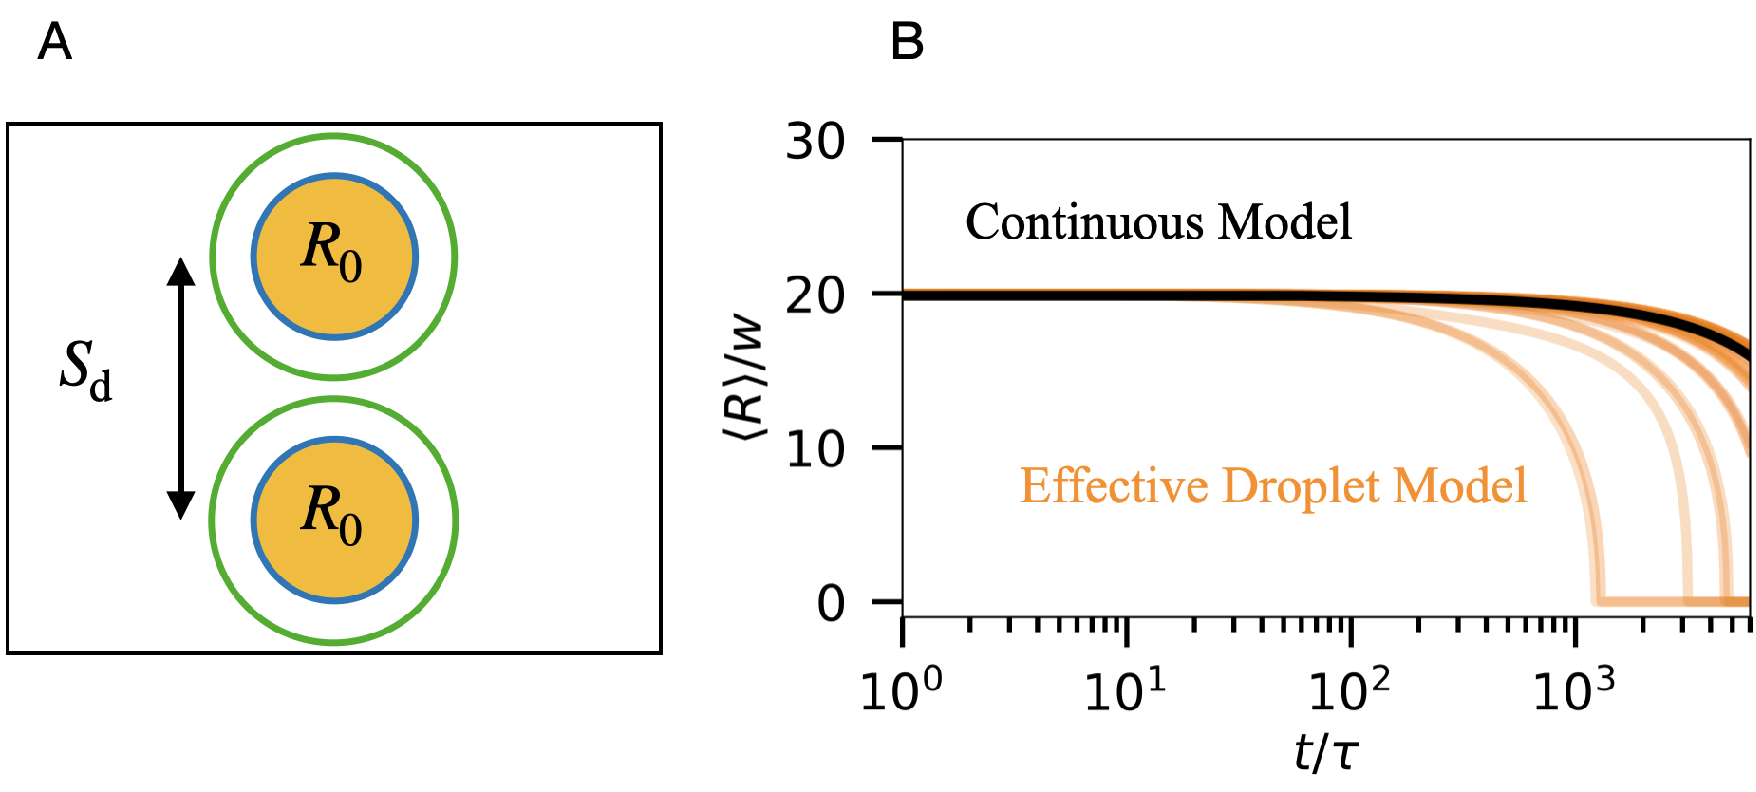
\includegraphics[scale=0.5]{MainContent/Figures/droplet_pair_schematic.pdf}
\caption{
\textbf{Schematics of the test-case (A) and typical behaviour of the effective droplet model for varying simulation parameters (B).}
(A) Two droplets with radii $R_0 = 20 w$ are placed with their centers $S_\mathrm{d} = 10 R_0$ apart in an empty background, $\phiOut(\vec{r}, t=0) = 0$, with their shells (in green).
(B) Mean droplet size $\langle R \rangle$ as a function of time for simulations using the continuous model (in black) and for varying simulation parameters for the effective droplet model (in orange).
$\langle R \rangle$ shows drastically different behaviour for some simulation parameters (orange lines) for the effective droplet model when compared to the continuous model (black line), thus highlighting the importance of choosing optimum values of simulation parameters for the effective droplet model.  
\mbox{(A, B)}
The continuous model simulations are performed in an azimuthally symmetric cylindrical domain of bounds $r,z \in [0, 682 w]$ with a spatial discretization of $0.5w$.
Effective simulations used a $3$-dimensional cubic domain of size $L = [0, 1000 w]^3$ with $l_{\gamma, \mathrm{in}} = 0.166 w$ and the simulation parameters were varied from uniformly choosing $\dx \in [0.5R_0, 10R_0], \ds \in [0.25R_0, 2R_0]$ and $\ell \in [0.5R_0, 5R_0]$.
Additional model parameters are $s=0$, $\Lambda = w^2 / b \, \tau$, $\phi^{(0)}_\mathrm{out} = 0$, $\phi^{(0)}_\mathrm{in} = 1$, $\tau = w^2/D_\mathrm{out}$, and $w = 2 \sqrt{\kappa / b}$.
}
\label{fig:droplet_pair_schematics}
\end{figure}

We first simulate the droplet pair using the continuous model for a duration $T$ after which the droplets typically have shrunk by about $20\%$.
We then simulate our effective droplet model for the same time $T$ and compare the final radii of the droplets from both the simulations. 
The deviation of the mean droplet radius $\mean{R_*}$ of our effective model compared to the radius $\mean{R_\mathrm{CM}}$ of the continuous model allows us to determine the crucial simulation parameters $\dx$, $\ell$, and $\ds$.

\section{$\dx \approx \ds \approx \ell$ is an optimum choice for the simulation parameters}

We first quantify the effects of changing the shell thickness $\ell$ on the accuracy of the simulation.
We keep the background field discretization $\dx \approx R_0$, as we aim to capture the interaction on a droplet level.  
\figref{fig:shell_parameters}A shows the final mean radii of the droplets $\langle R_\ast \rangle$ obtained from the effective droplet model and $\mean{R_\mathrm{CM}}$ (gray dashed line) obtained from the continuous model for $\dx \approx \ds$.
We see that the error is less than $\pm 5\%$  between $\langle R_\ast \rangle$ and $\mean{R_\mathrm{CM}}$ for the choice of $\ell \approx R_0$.
Similarly, we now fix $\dx \approx \ell$; see \figref{fig:shell_parameters}B and see that the error is less than $\pm 5\%$  between $\langle R_\ast \rangle$ and $\mean{R_\mathrm{CM}}$ for the choice of $\ds \approx R_0$.

\begin{figure}[tb]
\centering
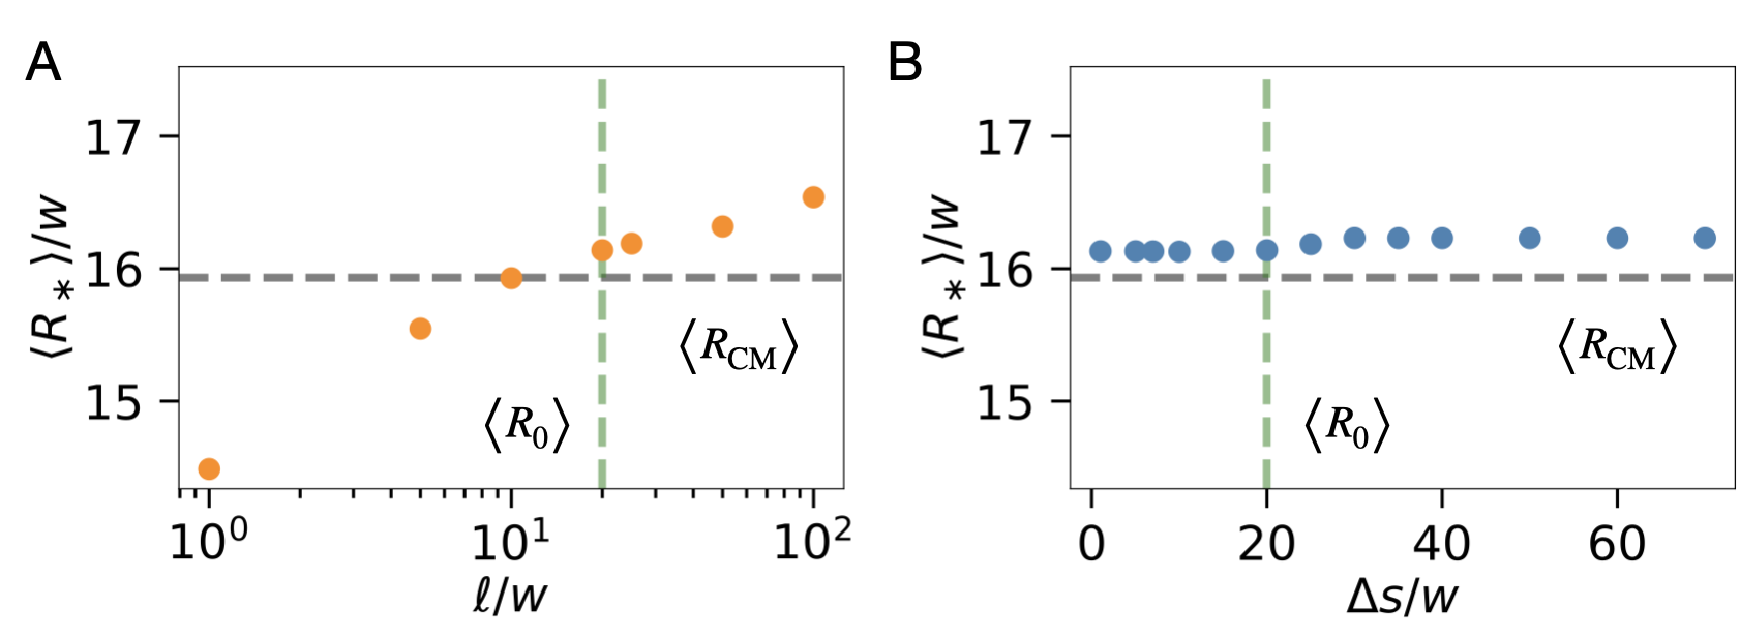
\includegraphics[scale=0.5]{MainContent/Figures/droplet_pair.pdf}
\caption{\textbf{Effect of shell thickness $\ell$ and sector size $\ds$ on simulations of a passive droplet pair.}
(A) Mean droplet size $\langle R_\ast \rangle$ as a function of $\ell$ (orange dots) for $\dx \approx \ds \approx R_0$ compared to the ground truth $\mean{R_\mathrm{CM}}$ (gray dashed line) obtained from the continuous model.
The choice $\ell \approx R_0$ (green dashed line) provides good agreement and the error between $\left \langle R_\mathrm{CM} \right \rangle$ (dotted grey line) and $\left \langle R_\ast \right \rangle$ is less than $\pm 5\%$.
(B) $\langle R_\ast \rangle$ as a function of $\ds$ (blue dots) for $\dx \approx \ell \approx R_0$ compared to $\mean{R_\mathrm{CM}}$, where the error between $\left \langle R_\mathrm{CM} \right \rangle$ (dotted grey line) and $\left \langle R_\ast \right \rangle$ is less than $\pm 5\%$.
Remaining parameters are specified in Fig. \ref{fig:droplet_pair_schematics}.
}
\label{fig:shell_parameters}
\end{figure}

Taken together, \figref{fig:shell_parameters} successfully shows that $\Delta x \approx \ell \approx \Delta s$ is a sensible choice for the parameters of our algorithm and leads to the best estimate of the droplet growth.
Finally, in order to ensure that our choice for the optimum parameters is independent of this particular test-case, we vary the initial radius of the droplets $R_0$ and their initial separation distance $S_\mathrm{d}$; see Appendix \ref{sec:RobustnessDropletPair}, as:

\begin{enumerate}
    \item $R_0 = 10w \mathrm{~and~} S_\mathrm{d} = 40w$.
    \item $R_0 = 10w \mathrm{~and~} S_\mathrm{d} = 100w$.
    \item $R_0 = 20w \mathrm{~and~} S_\mathrm{d} = 80w$.
\end{enumerate}

We follow the same procedure as before and simulate the droplet pair using the continuous model for a duration $T$ after which the droplets typically have shrunk by about $20\%$, then simulate our effective droplet model for the same time $T$ and compare the final radii of the droplets from both the simulations.

We report that our conclusion for the optimum choice of the simulation parameters largely remain unchanged with the above three test cases; see \figref{fig:robustness_test_case}, and hence we conclude that $\dx \approx \ds \approx \ell$ is an optimum choice for the simulation parameters, where $\dx$ is determined from the resolution of $\phiOut$ desired.
Finally the optimum time-step $\dt$ is then chosen using \Eqref{eqn:time_step} from the optimum set of parameters $[\dx, \ell, \ds]$.

To see how this choice of the optimum parameters affects accuracy and speed of the simulation, we present various simulation scenarios in the next chapter, which range from single droplets in an heterogeneous environment to droplet coarsening of large dilute emulsions.
We first simulate these systems with the effective droplet model using the optimum parameters and then show the effects of varying these parameters on droplet growth and drift. 

\section{Summary}

In Chapter \ref{chap:Chapter_3}, we formulated the numerical algorithm for the effective droplet model; given by (Algorithm \ref{alg:algorithm}), which evolved droplet dynamics according to \Eqsref{eqn:DropletDiscretized} and the background field volume fraction field $\phiOut$ according to \Eqref{eqn:RD_dilute}, with the time-step $\dt$ calculate from \Eqref{eqn:time_step}.

In this chapter, we discussed the various simulation parameters arising from the effective droplet model, namely $\dx, \ell, \ds$ and their effects on the simulation.
We then sought to find the values for optimum simulation parameters which best replicate droplet dynamics, when compared with simulations using the continuous model given by \Eqref{eqn:CHActive}.

We claimed that the optimum values for these simulation parameters are $\dx \approx \ell \approx \ds$.
To verify our claim, we simulated a synthetic test-case comprising of a pair of identical droplets shrinking in a vanishing background field. 

We first simulated the droplet pair using the continuous model for a duration $T$ after which the droplets typically had shrunk by about $20\%$.
We then simulated our effective droplet model for the same time $T$ and compared the final radii of the droplets from both the simulations.
The deviation of the mean droplet radius $\mean{R_*}$ of our effective model compared to the radius $\mean{R_\mathrm{CM}}$ of the continuous model allowed us to determine the optimum values of the simulation parameters which most faithfully model droplet dynamics as $\dx \approx \ell \approx \ds$ ; see \figref{fig:shell_parameters} and \figref{fig:robustness_test_case}.